\documentclass[12pt]{article}

\usepackage{fullpage}
\usepackage{multicol,multirow}
\usepackage{tabularx}
\usepackage{ulem}
\usepackage[utf8]{inputenc}
\usepackage[russian]{babel}
\usepackage{listings}
\usepackage{hyperref}
\usepackage{graphicx}
\DeclareGraphicsExtensions{.jpg}


\begin{document}

\section*{Лабораторная работа №\,3 по курсу криптографии}

Выполнил студент группы М8О-308Б-17 \textit{Иларионов Денис}.

\subsection*{Условие}
\begin{enumerate}
\item Строку в которой записано своё ФИО подать на вход в хеш-функцию ГОСТ Р 34.11-2012 (Стрибог). Младшие 4 бита выхода интерпретировать как число, которое в дальнейшем будет номером варианта. Процесс выбора варианта требуется отразить в отчёте.
\item Программно реализовать один из алгоритмов функции хеширования в соответствии с номером варианта. Алгоритм содержит в себе несколько раундов.
\item Модифицировать оригинальный алгоритм таким образом, чтобы количество раундов было настраиваемым параметром программы. в этом случае новый алгоритм не будет являться стандартом, но будет интересен для исследования.
\item Применить подходы дифференциального криптоанализа к полученным алгоритмам с разным числом раундов.
\item Построить график зависимости количества раундов и возможности различения отдельных бит при количестве раундов 1,2,3,4,5,... .
\item Сделать выводы.
\end{enumerate}

\subsection*{Метод решения}
Выбор варианта с помощью консольной утилиты, взятой из github.com/adegtyarev/streebog:\\
\includegraphics[width=\linewidth]{Screen1.jpg}\\

\textbf{Вариант 6: SHA-2}

Реализацию сиего алгоритма я решил поискать в интернете. Данная лабораторная работа меня в итоге побудила начать изучать питон, и сегодня я во время ее выполнения немного изучил синтаксис языка. На нем, действительно, очень удобно писать. А дело в том, что почти все реализации были на питоне. Вот и нашел я какую-то. После этого, я пытался во всем уже разобраться и сделать остальные задания.SHA-2 это более усовершенствованная версия SHA-1, его последователь. К данному алгоритму хеширования относится множество подтипов, такие, как SHA-224, SHA-256, SHA-384, SHA-512 и какие-то еще с делением, немного стремно выглядят. Я решил взять SHA-256, это наиболее распространенный тип этого алгоритма. Он работает следующим образом. Исходное сообщение после дополнения разбивается на блоки, каждый блок — на 16 слов. Алгоритм пропускает каждый блок сообщения через цикл с 64 раундами. На каждой итерации 2 слова преобразуются, функцию преобразования задают остальные слова. Результаты обработки каждого блока складываются, сумма является значением хеш-функции.

Инициализируются85 перменных:\\
$h0 := 0x6A09E667$ \\
$h1 := 0xBB67AE85$ \\
$h2 := 0x3C6EF372$ \\
$h3 := 0xA54FF53A$ \\
$h4 := 0x510E527F$ \\
$h5 := 0x9B05688C$ \\
$h6 := 0x1F83D9AB$ \\
$h7 := 0x5BE0CD19$ \\

На самом деле - это первые 32 бита дробных частей квадратных корней первых 8 простых чисел (от 2 до 19).
Также определяется таблица констант. Всего их - 64, поэтому SHA-256 не может выполнять более 64 раундов. Если, конечно, не дополнить эту таблицу еще значениями. Эти значения - первые 32 бита дробных частей кубических корней первых 64 простых чисел (от 2 до 311).

Мы обрабатываем сообщение предварительно в соответствие с определенными правилами. Далее, оно обрабатывается порциями по 512 бит - 16 слов по 32 бита. Генерируем дополнительные 48 слов. Инициализируем переменные и уже потом проводим раунды, в которых происходят циклические и логические сдвиги, xorы и прочие битовые операции. \\
\newline
После этого, мы складываем 8 хешей и получаем итоговое значение хеша. Если представить его в виде текста - 64 символа. В любом случае, каким бы ни было коротким или длинным исходное сообщение.\\
\newline
Основной цикл в каждом раунде:\\
$sum00$ := (a rotr 2) xor (a rotr 13) xor (a rotr 22) \\
$Ma$ := (a and b) xor (a and c) xor (b and c) \\
$t2$ := sum0 + Ma \\
$sum01$ := (e rotr 6) xor (e rotr 11) xor (e rotr 25) \\
$Ch$ := (e and f) xor ((not e) and g) \\
$t1$ := h + sum01 + Ch + k[i] + w[i] \\

Далее:\\
$h := g$ \\
$g := f$ \\
$f := e$ \\
$e := d + t1$ \\
$d := c$ \\
$c := b$ \\
$b := a$ \\
$a := t1 + t2$ \\

Добавляем полученные значения к ранее вычисленному результату: \\
$h0 := h0 + a$ \\
$h1 := h1 + b$ \\
$h2 := h2 + c$ \\
$h3 := h3 + d$ \\
$h4 := h4 + e$ \\
$h5 := h5 + f$ \\
$h6 := h6 + g$ \\
$h7 := h7 + h$ \\ \\


Получаем итоговое значение хеша:
$digest = hash = h0 || h1 || h2 || h3 || h4 || h5 || h6 || h7$ \\
|| - конкатенация (склеивание) битов.\\

\par
Реализация проходит все юнит тесты. Однако, изначальная версия, которую я нашел не проходила их. Была одна проблемка, а именно, что иногда длина хеша составляла не 64 символа, а меньше. Позже, я понял, в чем дело и исправил немного чужой код. А именно, проблема была в том, что в той реализации не учитывались ведущие нули в блоках. Я сделал тест в файле testing.py, который написал я полностью сам. Задается рандомное слово. Вычисляется хеш "моей" функцией и функцией, которая уже встроена в питоне в модуле hashlib. Если хеши равны, то к значению прибавляется 1. Как можно видеть дальше, значения всегда совпадали. \par
\begin{verbatim}
>>> checkingOK(5)  
'OK tests: 5/5'  
>>> checkingOK(10)  
'OK tests: 10/10'  
>>> checkingOK(50)  
'OK tests: 50/50'  
>>> checkingOK(100)  
'OK tests: 100/100'  
>>> checkingOK(500)  
'OK tests: 500/500'  
\end{verbatim}
\par
Далее были применены подходы дифференциального криптоанализа к полученной хеш-функции. Я генерирую рандомную строку заданной длины. Затем рандомно меняю последнюю букву и сравниваю хеши. Считаю несовпадения. Есть два вида подсчета, в зависимости от длины слова и вне зависимости. Дело в том, что я заметил, что чем длиннее слово, тем слабее различаются хеши при их одинаковом изменении. Вот начало листинга, а далее, я приведу диаграммы. На первой диаграмме - без учета длины слов, на второй - с ее учетом.\par
\begin{verbatim}
>>> cryptoAnalysis(0, 100, 0)
Rounds: 0 = 0
Rounds: 1 = 10
Rounds: 2 = 61
Rounds: 3 = 180
Rounds: 4 = 343
Rounds: 5 = 527
Rounds: 6 = 760
Rounds: 7 = 901
Rounds: 8 = 993
Rounds: 9 = 1062
Rounds: 10 = 1084
Rounds: 11 = 1087
Rounds: 12 = 1069
Rounds: 13 = 1101
................
\end{verbatim}

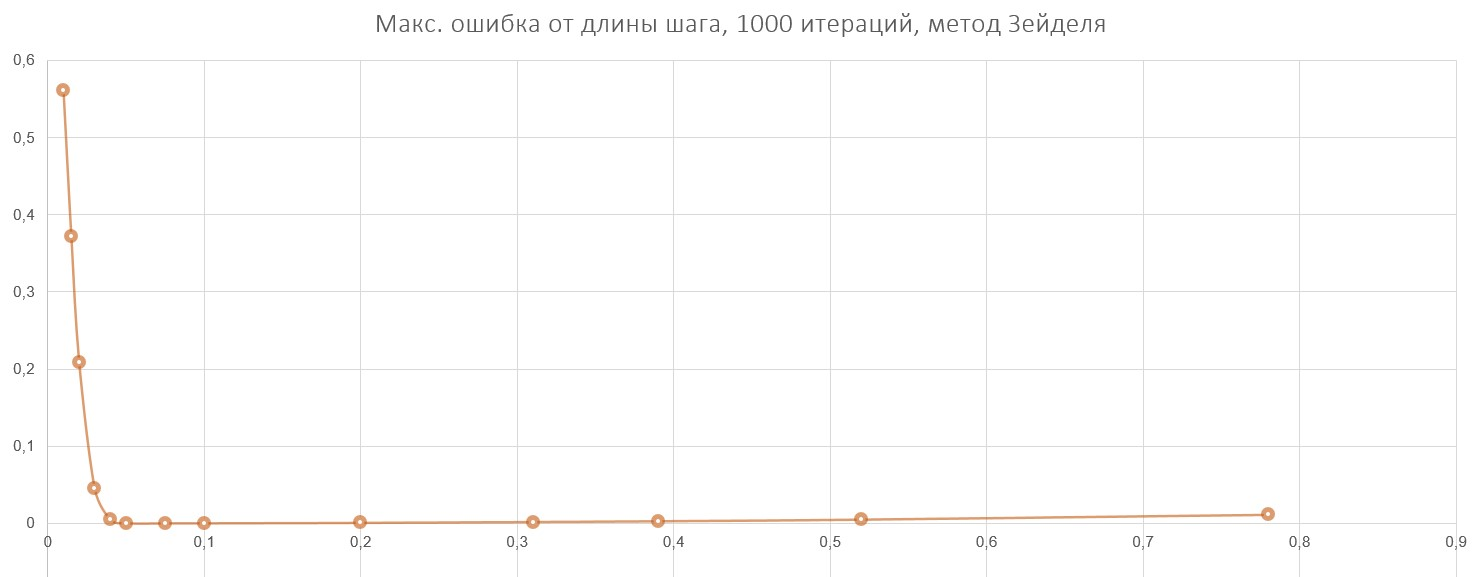
\includegraphics[width=\linewidth]{Graph1.jpg}\\
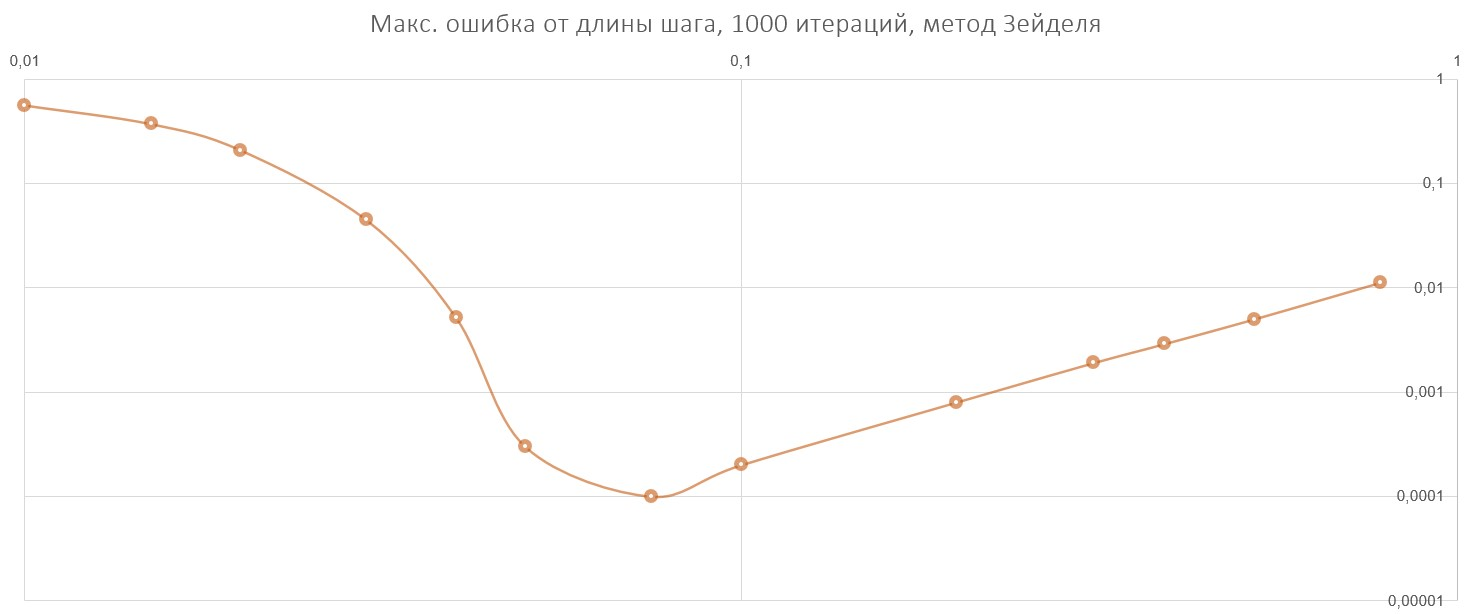
\includegraphics[width=\linewidth]{Graph2.jpg}\\

Мы видим резкие скачки примерно с 13 по 17 количество раундов. Затем примерно с 25 до 30. Затем, функция идет плавно, иногда даже отклоняется вниз от среднего значения. Это можно объяснить тем, что тесты я выбрал разные. Сначала 3 теста с длиной слова = 2, потом 4 теста с длиной слова = 5, затем 5 тестов с длиной слова = 10, 6 тестов с длиной слова = 20, 7 тестов с длиной 50, 10 с длиной 100 и 15 с длиной 500. И только при достаточном количестве раундов хеши строк такой длины с одним разным символом будут больше и больше различаться. Как я заметил позже, то хеши слов длиной 500 при изменении 1 символа вообще не отличаются, даже если брать максимальные, для SHA-256, 64 раунда. Поэтому, более эффективно использовать около 30 раундов, если работать со строками не длиннее 100 символов. Чем меньше раундов, тем быстрее будет работать программа, а при таких данных между 30 и 60 раундами разницы эффективности почти нет, только работает дольше...
\subsection*{Результат работы программы}
\begin{lstlisting}
>>> sha_256("Nosik")
'222ce3fee70f7ca09e387804ff3595fa864e92263f3ccb5915633561df5fdf91'
>>> sha_256("Noski")
'ea7b9957679f6a4e643caa3f8dc5a204d2df1692eacf1bc01e4f7c144408eddb'
>>> sha_256("Nosik", 3)
'df70be72811de8b386e6ef280f59dba17eb1c6bda201330a06bb2fb6acef1f98'
>>> sha_256("Noski", 3)
'2b844db0f74dbfac86e6ef2a0f59dba18403ad909841320806bb2fb8acef1f98'
>>> stringDiff(sha_256("Nosik"), sha_256("Noski"))
58
>>> stringDiff(sha_256("Nosik", 3), sha_256("Noski", 3))
30
>>> stringDiff(sha_256("Nosik", 2), sha_256("Noski", 2))
15
>>> stringDiff(sha_256("Nosik", 1), sha_256("Noski", 1))
2
>>> sha_256("Nosik", 1)
'b481e21d257194ecf7d6a1f7e1bee8ac3845a88aec13bb0bba8942377b64a6c4'
>>> sha_256("Noski", 1)
'b481e21f257194ecf7d6a1f7e1bee8ac3845a88cec13bb0bba8942377b64a6c4'
\end{lstlisting}

\subsection*{Выводы}
Во время выполнения данной лабораторной работы, я больше изучил питон, чем что-либо другое) Ну а если серьезно, то я познакомился с хеш-функциями, а именно с функциями, подобными SHA-2. С помощью таких функций можно зашифровать любое сообщение. Однако, есть очень большой минус, а именно, что непосредственно из хеш функций нельзя вывести ту строку, из которой она получилась. Если бы такое было бы возможно, то подобные хеш функции были бы просто невероятно эффективным инструментом сокращения текста. Потому что из любой строки получается хеш, который в виде строки для SHA-256 занимает ровно 64 символа. Однако, у хеш-функций есть хорошее применение. Есть специальные базы данных, где хранятся такие хеши и уже по ним можно получить и сообщение. Очень хорошее применение таких функций можно использовать в сохранениях в игре. Игрок может сохранить все данные, получив небольшой хеш. А уже он поступает на сервер вместе с данными. И при этом игрок никак не сможет обхитрить и взломать сохранение, потому что данные по этому хешу на сервере. Также можно сохранять какие-то важные данные и хранить лишь хеши. Есть очень много применений для таких функций, я считаю, так что, данная лабораторная оказалась вполне важной. С хеш функциями я еще познакомился на 1 курсе во время олимпиадного программирования. Там использовались простые хеш функции, которые были равны произведению чисел с определенным остатком.

\subsection*{Листинг программного кода}
sha256.py
\begin{lstlisting}[language=Python]
initial_hash_values=[
'6a09e667','bb67ae85','3c6ef372','a54ff53a',
'510e527f','9b05688c','1f83d9ab','5be0cd19'
]

sha_256_constants=[
'428a2f98','71374491','b5c0fbcf','e9b5dba5',
'3956c25b','59f111f1','923f82a4','ab1c5ed5',
'd807aa98','12835b01','243185be','550c7dc3',
'72be5d74','80deb1fe','9bdc06a7','c19bf174',
'e49b69c1','efbe4786','0fc19dc6','240ca1cc',
'2de92c6f','4a7484aa','5cb0a9dc','76f988da',
'983e5152','a831c66d','b00327c8','bf597fc7',
'c6e00bf3','d5a79147','06ca6351','14292967',
'27b70a85','2e1b2138','4d2c6dfc','53380d13',
'650a7354','766a0abb','81c2c92e','92722c85',
'a2bfe8a1','a81a664b','c24b8b70','c76c51a3',
'd192e819','d6990624','f40e3585','106aa070',
'19a4c116','1e376c08','2748774c','34b0bcb5',
'391c0cb3','4ed8aa4a','5b9cca4f','682e6ff3',
'748f82ee','78a5636f','84c87814','8cc70208',
'90befffa','a4506ceb','bef9a3f7','c67178f2'
]

def bin_return(dec):
    return(str(format(dec,'b')))

def bin_8bit(dec):
    return(str(format(dec,'08b')))

def bin_32bit(dec):
    return(str(format(dec,'032b')))

def bin_64bit(dec):
    return(str(format(dec,'064b')))

def hex_return(dec):
    return(str(format(dec,'x')))

def dec_return_bin(bin_string):
    return(int(bin_string,2))

def dec_return_hex(hex_string):
    return(int(hex_string,16))

def L_P(SET,n):
    to_return=[]
    j=0
    k=n
    while k<len(SET)+1:
        to_return.append(SET[j:k])
        j=k
        k+=n 
    return(to_return)

def s_l(bit_string):
    bit_list=[]
    for i in range(len(bit_string)):
        bit_list.append(bit_string[i])
    return(bit_list)

def l_s(bit_list):
    bit_string=''
    for i in range(len(bit_list)):
        bit_string+=bit_list[i]
    return(bit_string)

def rotate_right(bit_string,n):
    bit_list = s_l(bit_string)
    count=0
    while count <= n-1:
        list_main=list(bit_list)
        var_0=list_main.pop(-1)
        list_main=list([var_0]+list_main)
        bit_list=list(list_main)
        count+=1
    return(l_s(list_main))

def shift_right(bit_string,n):
    bit_list=s_l(bit_string)
    count=0
    while count <= n-1:
        bit_list.pop(-1)
        count+=1
    front_append=['0']*n
    return(l_s(front_append+bit_list))

def mod_32_addition(input_set):
    value=0
    for i in range(len(input_set)):
        value+=input_set[i]
    mod_32 = 4294967296
    return(value%mod_32)

def xor_2str(bit_string_1,bit_string_2):
    xor_list=[]
    for i in range(len(bit_string_1)):
        if bit_string_1[i]=='0' and bit_string_2[i]=='0':
            xor_list.append('0')
        if bit_string_1[i]=='1' and bit_string_2[i]=='1':
            xor_list.append('0')
        if bit_string_1[i]=='0' and bit_string_2[i]=='1':
            xor_list.append('1')
        if bit_string_1[i]=='1' and bit_string_2[i]=='0':
            xor_list.append('1')
    return(l_s(xor_list))

def and_2str(bit_string_1,bit_string_2):
    and_list=[]
    for i in range(len(bit_string_1)):
        if bit_string_1[i]=='1' and bit_string_2[i]=='1':
            and_list.append('1')
        else:
            and_list.append('0')

    return(l_s(and_list))

def or_2str(bit_string_1,bit_string_2):
    or_list=[]
    for i in range(len(bit_string_1)):
        if bit_string_1[i]=='0' and bit_string_2[i]=='0':
            or_list.append('0')
        else:
            or_list.append('1')
    return(l_s(or_list))

def not_str(bit_string):
    not_list=[]
    for i in range(len(bit_string)):
        if bit_string[i]=='0':
            not_list.append('1')
        else:
            not_list.append('0')
    return(l_s(not_list))

'''
SHA-256 Specific Functions:
'''

def Ch(x,y,z):
    return(xor_2str(and_2str(x,y),and_2str(not_str(x),z)))

def Maj(x,y,z):
    return(xor_2str(xor_2str(and_2str(x,y),and_2str(x,z)),and_2str(y,z)))

def e_0(x):
    return(xor_2str(xor_2str(rotate_right(x,2),rotate_right(x,13)),rotate_right(x,22)))

def e_1(x):
    return(xor_2str(xor_2str(rotate_right(x,6),rotate_right(x,11)),rotate_right(x,25)))

def s_0(x):
    return(xor_2str(xor_2str(rotate_right(x,7),rotate_right(x,18)),shift_right(x,3)))

def s_1(x):
    return(xor_2str(xor_2str(rotate_right(x,17),rotate_right(x,19)),shift_right(x,10)))

def message_pad(bit_list):
    pad_one = bit_list + '1'
    pad_len = len(pad_one)
    k=0
    while ((pad_len+k)-448)%512 != 0:
        k+=1
    back_append_0 = '0'*k
    back_append_1 = bin_64bit(len(bit_list))
    return(pad_one+back_append_0+back_append_1)

def message_bit_return(string_input):
    bit_list=[]
    for i in range(len(string_input)):
        bit_list.append(bin_8bit(ord(string_input[i])))
    return(l_s(bit_list))

def message_pre_pro(input_string):
    bit_main = message_bit_return(input_string)
    return(message_pad(bit_main))

def message_parsing(input_string):
    return(L_P(message_pre_pro(input_string),32))

def message_schedule(index,w_t):
    new_word = bin_32bit(mod_32_addition([int(s_1(w_t[index-2]),2),int(w_t[index-7],2),int(s_0(w_t[index-15]),2),int(w_t[index-16],2)]))
    return(new_word)

'''
This example of SHA_256 works for an input string <56 characters.
'''

def sha_256(input_string, rounds = 64):
    w_t=message_parsing(input_string)
    a=bin_32bit(dec_return_hex(initial_hash_values[0]))
    b=bin_32bit(dec_return_hex(initial_hash_values[1]))
    c=bin_32bit(dec_return_hex(initial_hash_values[2]))
    d=bin_32bit(dec_return_hex(initial_hash_values[3]))
    e=bin_32bit(dec_return_hex(initial_hash_values[4]))
    f=bin_32bit(dec_return_hex(initial_hash_values[5]))
    g=bin_32bit(dec_return_hex(initial_hash_values[6]))
    h=bin_32bit(dec_return_hex(initial_hash_values[7]))
    for i in range(0, rounds):
        if i <= 15: 
            t_1=mod_32_addition([int(h,2),int(e_1(e),2),int(Ch(e,f,g),2),int(sha_256_constants[i],16),int(w_t[i],2)])
            t_2=mod_32_addition([int(e_0(a),2),int(Maj(a,b,c),2)])
            h=g
            g=f
            f=e
            e=mod_32_addition([int(d,2),t_1])
            d=c
            c=b
            b=a 
            a=mod_32_addition([t_1,t_2])
            a=bin_32bit(a)
            e=bin_32bit(e)
        if i > 15:
            w_t.append(message_schedule(i,w_t))
            t_1=mod_32_addition([int(h,2),int(e_1(e),2),int(Ch(e,f,g),2),int(sha_256_constants[i],16),int(w_t[i],2)])
            t_2=mod_32_addition([int(e_0(a),2),int(Maj(a,b,c),2)])
            h=g
            g=f
            f=e
            e=mod_32_addition([int(d,2),t_1])
            d=c
            c=b
            b=a 
            a=mod_32_addition([t_1,t_2])
            a=bin_32bit(a)
            e=bin_32bit(e)
    hash_0 = mod_32_addition([dec_return_hex(initial_hash_values[0]),int(a,2)])
    hash_1 = mod_32_addition([dec_return_hex(initial_hash_values[1]),int(b,2)])
    hash_2 = mod_32_addition([dec_return_hex(initial_hash_values[2]),int(c,2)])
    hash_3 = mod_32_addition([dec_return_hex(initial_hash_values[3]),int(d,2)])
    hash_4 = mod_32_addition([dec_return_hex(initial_hash_values[4]),int(e,2)])
    hash_5 = mod_32_addition([dec_return_hex(initial_hash_values[5]),int(f,2)])
    hash_6 = mod_32_addition([dec_return_hex(initial_hash_values[6]),int(g,2)])
    hash_7 = mod_32_addition([dec_return_hex(initial_hash_values[7]),int(h,2)])
    string_hash_0 = "00000000"[0:(8 - len(hex_return(hash_0)))] + hex_return(hash_0)
    string_hash_1 = "00000000"[0:(8 - len(hex_return(hash_1)))] + hex_return(hash_1)
    string_hash_2 = "00000000"[0:(8 - len(hex_return(hash_2)))] + hex_return(hash_2)
    string_hash_3 = "00000000"[0:(8 - len(hex_return(hash_3)))] + hex_return(hash_3)
    string_hash_4 = "00000000"[0:(8 - len(hex_return(hash_4)))] + hex_return(hash_4)
    string_hash_5 = "00000000"[0:(8 - len(hex_return(hash_5)))] + hex_return(hash_5)
    string_hash_6 = "00000000"[0:(8 - len(hex_return(hash_6)))] + hex_return(hash_6)
    string_hash_7 = "00000000"[0:(8 - len(hex_return(hash_7)))] + hex_return(hash_7)
    final_hash = (string_hash_0 +
                  string_hash_1 +
                  string_hash_2 +
                  string_hash_3 +
                  string_hash_4 +
                  string_hash_5 +
                  string_hash_6 +
                  string_hash_7)
    return(final_hash)


\end{lstlisting}

testing.py
\begin{lstlisting}[language=Python]
import random
import string
import logging
import hashlib
import bitstring
import sha256
from sha256 import *
from hashlib import sha256

def genRandStr(size):
    k = ""
    for i in range(size):
        k += random.choice('abcdefghijklmnopqrstuvwxyzABCDEFGHIJKLMNOPQRSTUVWXYZ')
    return k


def changeLast(string):
    lastS = string[- 1]
    prevPart = string[:- 1]
    randomList = 'abcdefghijklmnopqrstuvwxyzABCDEFGHIJKLMNOPQRSTUVWXYZ'
    ind = randomList.index(lastS)
    newList = randomList[:ind] + randomList[(ind+1):]
    return prevPart + random.choice(newList)


def origSha256(string):
    return sha256(string.encode('utf-8')).hexdigest()


def checkingOK(tests):
    okTests = 0
    for i in range(tests):
        theString = genRandStr(random.randrange(3, 50))
        ans1 = sha_256(theString)
        ans2 = origSha256(theString)
        if ans1 == ans2 : okTests += 1
    return "OK tests: " + str(okTests) + "/" + str(tests)



def stringDiff(str1, str2):
    diff = 0
    minL = min(len(str1), len(str2))
    maxL = max(len(str1), len(str2))
    diff += maxL - minL
    for i in range(minL):
        if str1[i] != str2[i]:
            diff += 1
    return diff



def cryptoAnalysis(start, end, mults = 0):
    for k in range(start, end+1):
        score = 0
        #3 строки из 2 символов
        for i in range(3):
            newS = genRandStr(2)
            newS2 = changeLast(newS)
            sha1 = sha_256(newS, k)
            sha2 = sha_256(newS2, k)
            score += stringDiff(sha1, sha2) * (1 + (mults*1))

        #4 строки из 5 символов
        for i in range(4):
            newS = genRandStr(5)
            newS2 = changeLast(newS)
            sha1 = sha_256(newS, k)
            sha2 = sha_256(newS2, k)
            score += stringDiff(sha1, sha2) * (1 + (mults*4))

        #5 строк из 10 символов
        for i in range(5):
            newS = genRandStr(10)
            newS2 = changeLast(newS)
            sha1 = sha_256(newS, k)
            sha2 = sha_256(newS2, k)
            score += stringDiff(sha1, sha2) * (1 + (mults*9))

        #6 строк из 20 символов
        for i in range(6):
            newS = genRandStr(20)
            newS2 = changeLast(newS)
            sha1 = sha_256(newS, k)
            sha2 = sha_256(newS2, k)
            score += stringDiff(sha1, sha2) * (1 + (mults*19))

        #7 строк из 50 символов
        for i in range(7):
            newS = genRandStr(50)
            newS2 = changeLast(newS)
            sha1 = sha_256(newS, k)
            sha2 = sha_256(newS2, k)
            score += stringDiff(sha1, sha2) * (1 + (mults*49))

        #10 строк из 100 символов
        for i in range(10):
            newS = genRandStr(100)
            newS2 = changeLast(newS)
            sha1 = sha_256(newS, k)
            sha2 = sha_256(newS2, k)
            score += stringDiff(sha1, sha2) * (1 + (mults*99))

        #15 строк из 500 символов
        for i in range(15):
            newS = genRandStr(500)
            newS2 = changeLast(newS)
            sha1 = sha_256(newS, k)
            sha2 = sha_256(newS2, k)
            score += stringDiff(sha1, sha2) * (1 + (mults*499))

        
        print("Rounds: " + str(k) + " = " + str(score))
    
\end{lstlisting}

\end{document}